\documentclass[main.tex]{subfiles}
\begin{document}


\section{Some Remarks on Gravity in 2+1 Dimensions}

Gravity in $2+1$ dimensions is a special example of a classical theory that is difficult to quantize properly, at least if we wish to admit the presence of matter. One can think of scalar (spin zero) particles whose only interactions consist of the exchange of a gravitational force. The classical theory $[99,105,124]$ suggests that it can be quantized, but something very special happens [ 107] , as we shall illustrate now. The Einstein equations for regions without matter particles read
$$
R_{\mu \nu}=0
$$
but in $2+1$ dimensions, we can write
$$
\begin{aligned}
S^{\alpha \beta} &=S^{\beta \alpha}=\frac{1}{4} \varepsilon^{\alpha \mu \nu} \varepsilon^{\beta \kappa \lambda} R_{\mu \nu \kappa \lambda}, \quad R_{\mu \nu \kappa \lambda}=\varepsilon_{\mu \nu \alpha} \varepsilon_{\kappa \lambda \beta} S^{\alpha \beta} \\
R_{\mu \nu} &=g_{\mu \nu} S^{\alpha \alpha}-S_{\mu \nu}, \quad S_{\mu \nu}=-R_{\mu \nu}+\frac{1}{2} R g_{\mu \nu}
\end{aligned}
$$
Consequently, Eq. (A.1) also implies that the Riemann tensor $R_{\mu v k \lambda}$ vanishes. Therefore, matter-free regions are flat pieces of space-time (which implies that,
in $2+1$ dimensions, there are no tidal forces. When a particle is present, however, $R_{\mu v}$ does not vanish, and therefore a particle is a local, topological defect. One finds that a particle, when at rest, cuts out a wedge from the 2 -dimensional space surrounding it, turning that 2 -space into a cone, and the deficit angle of the excised region is proportional to the mass: In convenient choices of the units, the total wedge angle is exactly twice the mass $\mu$ of the particle. When the particle moves, we choose to orient the wedge with its deficit angle such that the particle moves in the direction of the bisector of the angle. Then, if we ask for the effect of the associated Lorentz transformation, we see that the wedge is Lorentz contracted. This is illustrated in Fig. A.1, where the crosses and circles indicate which points are identified when we follow a loop around the particle. We see that, because we chose the particle to move along the bisector, there is no time shift at this identification, otherwise, there would have been. This way we achieve that the surrounding space can be handled as a Cauchy surface for other particles that move around.

\begin{figure}[ht]
	\begin{center}
		\scalebox{0.4}{
		   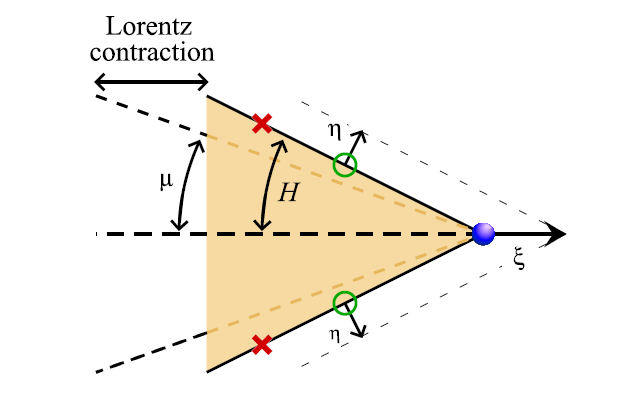
\includegraphics{images/img_A_1.png}
		}
		\caption{
		\label{iA.1} The angle cut out of space when a particle moves with velocity $\xi$. See text}
	\end {center}
\end {figure}


Some arithmetic shows that, if the particle's velocity is defined as tanh $\xi,$ the Lorentz contraction factor is cosh $\xi,$ and the opening angle $H$ of the moving particle is given by
$$
\tan H=\cosh \xi \tan \mu
$$
If $\eta$ is the velocity of the seam between the two spaces (arrow in Fig. A.1), then we find
$$
\begin{aligned}
\tanh \eta &=\sin H \tanh \xi \\
\cos \mu &=\cos H \cosh \eta \\
\sinh \eta &=\sin \mu \sinh \xi
\end{aligned}
$$
Equation (A.3) gives a relation between $H$ and $\mu$ that turns into the usual relation between mass in motion and energy in the weak gravity limit, while deficit angles such as $H$ are additive and conserved. Therefore, we interpret $H$ as the energy of the moving particle, in the presence of gravity.

In Ref. $[107],$ we argued that, taking $\mu$ to be constant, $\mathrm{d}(\cos H \cosh \eta)=0,$ so that
$$
-\sin H \cosh \eta \mathrm{d} H+\cos H \sinh \eta \mathrm{d} \eta=0, \quad \frac{\partial H}{\partial \eta}=\frac{\tanh \eta}{\tan H}
$$
Furthermore, it was derived that we can make tessellations of Cauchy surfaces using configurations such as in Fig. A. 1 in combination with vertices where no particles are residing, so that the Cauchy surface is built from polygons. The edges $L_{i}$ where one polygon is connected to another either end in one of these auxiliary vertices or one of the physical particles. We can then calculate how the lengths of the edges $L_{i}$ grow or shrink.

Both end points of a boundary line make the line grow or shrink with independent velocities, but the orthogonal components are the same. To define these unambiguously, we take a point such as the small circle in Fig. A.1, which moves in a direction orthogonal to the seam. We now see that our particle gives a contribution to $dL/dt$ 

equal to
$$
\left.\frac{\mathrm{d} L}{\mathrm{d} t}\right|_{\xi}=\tanh \xi \cos H
$$
Combining this with Eqs. (A.4) and (A.7), one finds
$$
\left.\frac{\mathrm{d} L}{\mathrm{d} t}\right|_{\xi}=\frac{\tanh \eta}{\tan H}=\frac{\partial H}{\partial \eta}
$$
Furthermore, the Hamiltonian does not depend on $L,$ while $\eta$ does not depend on time, so that
$$
\frac{\mathrm{d} \eta}{\mathrm{d} t}=-\frac{\partial H}{\partial L}=0
$$
These last two equations can be seen as the Hamilton equations for $L$ and $\eta$ This means that $\eta$ and $L$ are canonically associated with one another. If there are many polygons connected together with seams $L_{i},$ moving with transverse velocities tanh $\eta_{i},$ then we obtain Hamiltonian equations for their time dependence, with Poisson brackets
$$
\left\{L_{i}, \eta_{j}\right\}=\delta_{i j}
$$
Thus, the lengths $L_{i}$ are like positions and the $\eta_{i}$ are like the associated momenta. This clearly suggests that all one needs to do to obtain the quantum theory is to postulate that these Poisson brackets are replaced by commutators.

\subsection{Discreteness of Time}

There is, however, a serious complication, due to the nature of our Hamiltonian. If we have many particles, all adding deficit angles to the shape of our Cauchy surface, one can easily see what might happen: $^{2}$
If the total energy due to matter particles exceeds the value $\pi$, the universe will close into itself, allowing only the value $2 \pi$ for its total Hamiltonian,
assuming that the universe is simply connected. Thus, the question arises what it means to vary the Hamiltonian with respect to $\eta^{\prime}$ s, as in Eq. (A.9).

There is a way to handle this question: consider some region $X$ in the universe $\Omega$, and ask how it evolves with respect to data in the rest of the universe, $\Omega \backslash X .$ The problem is then to define where the boundary between the two regions $X$ and $\Omega \backslash X$ is.

An other peculiar feature of this Hamiltonian is that it is defined as an angle (even if it might exceed the value $\pi ;$ it cannot exceed $2 \pi$ ). In the present work, we became quite familiar with Hamiltonians that are actually simple angles: this means that their conjugate variable, time, is discrete. The well-defined object is not the Hamiltonian itself, but the evolution operator over one unit of time: $U=e^{-i H}$ Apparently, what we are dealing with here, is a world where the evolution goes in discretized steps in time.

The most remarkable thing however, is that we cannot say that the time for the entire universe is discrete. Global time is a meaningless concept, because gravity is
a diffeomorphism invariant theory. Time is just a coordinate, and physical states are invariant under coordinate transformations, such as a global time translation. It is
in regions where matter is absent where we have local flatness, and only in those regions, relative time is well-defined, and as we know now, discrete. Because of the absence of a global time concept, we have no Schrödinger equation, or even a discrete time-step equation, that tells us how the entire universe evolves.

Suppose we split the universe $\Omega$ into two parts, $X$ and $\Omega \backslash X .$ Then the edges
$L_{i}$ in $X$ obey a Schrödinger equation regarding their dependence on a relative time variable $t$ (it is relative to time in $\Omega \backslash X$ ). The Schrödinger equation is derived from Eq. (A.5), where now $H$ and $\eta$ are operators:
$$
\eta=-i \frac{\partial}{\partial L}, \quad H=i \frac{\partial}{\partial t}
$$
If the wave function is $\psi(L, t),$ then
$$
(\cos H) \psi(L, t)=\frac{1}{2}(\psi(L, t+1)+\psi(L, t-1))
$$

and the action of $1 / \cosh \eta$ on $\psi(L, t)$ can be found by Fourier transforming this operator:
$$
(\cosh \eta)^{-1} \psi(L, t)=\int_{-\infty}^{\infty} \mathrm{d} y \frac{1}{2 \cosh (\pi y / 2)} \psi(L+y, t)
$$
So, the particle in Fig. A. 1 obeys the Schrödinger equation following from Eq. (A.5):
$$
\psi(L, t+1)+\psi(L, t-1)=\int_{-\infty}^{\infty} \mathrm{d} y \frac{\cos \mu}{\cosh (\pi y / 2)} \psi(L+y, t)
$$
The problem with this equation is that it involves all $L$ values, while the polygons forming the tessellation of the Cauchy surface, whose edge lengths are given by the $L_{i},$ will have to obey inequalities, and therefore it is not clear to us how to proceed from here. In Ref. [ 107] we tried to replace the edge lengths $L_{i}$ by the particle coordinates themselves. It turns out that they indeed have conjugated momenta that form a compact space, so that these coordinates span some sort of lattice, but this is not a rectangular lattice, and again the topological constraints were too difficult to handle.

The author now suspects that, in a meaningful theory for a system of this sort, we must require all dynamical variables to be sharply defined, so as to be able to define their topological winding properties. Now that would force us to search for deterministic, classical models for $2+1$ dimensional gravity. In fact, the difficulty of formulating a meaningful 'Schrödinger equation' for a $2+1$ dimensional universe, and the insight that this equation would (probably) have to be deterministic, was one of the first incentives for this author to re-investigate deterministic quantum mechanics as was done in the work reported about here: if we would consider any classical model for $2+1$ dimensional gravity with matter (which certainly can be formulated in a neat way), declaring its classical states to span a Hilbert space in the sense described in our work, then that could become a meaningful, unambiguous quantum system $[99,105,124]$

Our treatment of gravity in $2+1$ dimensions suggests that the space-time metric and the gravitational fields should be handled as being a set of beables. Could we do the same thing in $3+1$ dimensions? Remember that the source of gravitational fields, notably the energy density, is not a beable, unless we decide that the gravitational fields generated by energies less than the Planck energy, are negligible anyway (in practice, these fields are too feeble to detect), while our considerations regarding the discretized Hamiltonian, Sects. 19.2 and $19.3,$ suggest the one can define large, discretized, amounts of energy that indeed behave as beables.

Consider a $3+1$ dimensional gravitating system, where one of the space dimensions is compactified. It will then turn into a $2+1$ dimensional world, which we just argued should be subject to the CAI. Should our universe not be regarded as just such a world in the limit where the compactification length of the third spacial dimension tends to infinity? We believe the answer is yes.





\subsection{}
\subsection{}
\subsection{}
\subsection{}
\subsection{}
\subsection{}
\subsection{}
\subsection{}




\begin{equation}\label{}
	
\end{equation}









\end{document}

